%-*-coding: utf-8-*-

\chapter{Описание технических аспектов реализации}
В данной главе будут представлены технические аспекты реализации лямбда-функций и функций высших порядков.
Будет показана техническая сложность и примененные подходы при решении поставленной задачи.

\section{Общий принцип работы}
Для начала необходимо рассмотреть общий принцип работы \verb|KPHP| и его архитектуру, также решить, как правильно подходить к решению данной задачи.
\verb|KPHP| -- состоит из двух основных частей:
\begin{enumerate}
\item компилятор -- занимается разбором написанного кода, построением абстрактного синтаксического дерева, анализом, трансляцией и выступает в качестве драйвера для компиляции оттранслированной программы;
\item рантайм -- библиотека необходимая для запуска скомпилированных программ, содержащая встроенные функции языка.
\end{enumerate}

\subsection{Принцип работы компилятора}
Компилятор запускается с 24 рабочими потоками, для ускорения выполнения работ, большинство из этапов конвейера работают параллельно, что значительно уменьшает время выполнения трансляции.
На рисунке \ref{fig:compiler_arch} наглядно показана упрощенная схема основных этапов работы.
Если переход между этапами обозначен стрелочкой -- это значит, что результат от предыдущего этапа сразу же передается на следующий.
Переходы же, имеющие круглый конец, означают, что необходимо дождаться выполнения всех предыдущих этапов во всех потоках выполнения перед тем, как продолжить.

\begin{figure}[H]
    \caption{Общий принцип работы компилятора}
    \label{fig:compiler_arch}
    \centering
    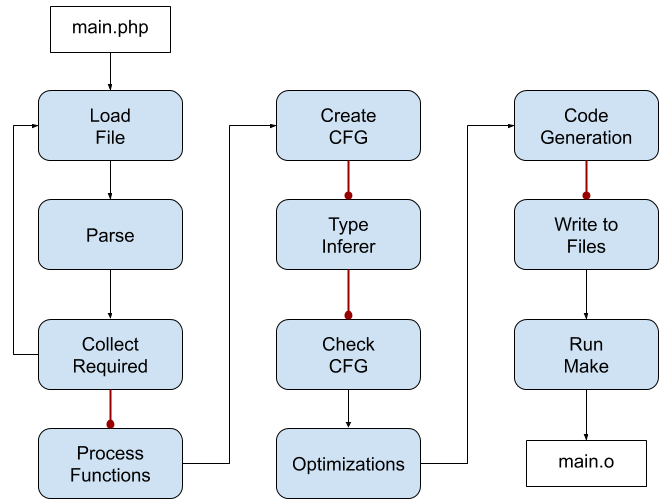
\includegraphics[width=\linewidth]{images/compiler_arch}
\end{figure}

Помимо множества аргументов, которые передаются на вход при запуске компилятора, будет интересно взглянуть только один -- это путь к файлу, который является отправной точкой для компиляции.
Данный файл передается в начало конвейера, на рисунке \ref{fig:compiler_arch} он имеет имя <<\verb|main.php|>>.
На этапе <<\verb|Load File|>> происходит полная загрузка переданного файла в память для дальнейшего разбора и анализа.
После чего в компиляторе происходит разбиение этого файла на токены и построение из них абстрактного синтаксического дерева для конкретного потока символов.
Имея построенное дерево разбора, можно понимать какие вершины встречаются и без труда выявить все зависимости, которые будут необходимы KPHP для дальнейшей работы.
Каждый файл, который является зависимостью для предыдущего пришедшего файла отправляется снова на стадию <<\verb|Load File|>> и все этапы повторяются с самого начала.

На вход следующего шага уже передаются только разобранные функции.
При прохождении через <<\verb|Process Functions|>>  функций, одна из основных задач расставить всем вершинам необходимые идентификаторы, соответствующие вызову другой функции.
Это важный этап, к которому уже должны быть разобраны все функции из других файлов, чтобы суметь проставить ссылки.
Далее происходит построение \verb|CFG| \cite{CFG}, необходимого для последующего анализа и оптимизаций.

Вывод типов для переменных, параметров функций, а также возвращаемых значений происходит на шаге <<\verb|Type Inferencer|>>.
В этот момент компилятор использует специальный файл -- <<\verb|functions.txt|>>, содержащий аннотирование встроенных функции, которые нужны программистам, разрабатывающим на языке \verb|KPHP|.
Так как в этом файле нет тела самих функций, мы вынуждены вводить свою аннотацию в данном случае.
Вывод типов для них опирается на то, что написано в данном файле.
Дальше необходимо проверять корректность и различные ограничения используя построенный \verb|CFG| и выведенные типы у вершин и пытаться оптимизировать наши функции.

После основных этапов получаются готовые деревья \verb|AST| для всех функций.
Осталось лишь сгенерировать их в текстовое представление для последующей записи в файлы.
Учитывая выведенные типы, надо определить, где необходимо печатать соответствующие типы выражений, а также в зависимости от вида вершины преобразовать в соответствующий код на языке C++.
Далее уже готовое текстовое представление, распределенное по файлам, необходимо записать на диск с нужным делением по директориям для ускорения дальнейшей сборки.

Последний из основных этапов, который будет рассмотрен -- это <<\verb|Run Make|>>.
На данном этапе смотрим на времена изменений файлов и понимаем какие зависимости нужно собрать заново.
Сборка происходит в несколько этапов:
\begin{enumerate}
  \item многопоточная компиляция каждой из единиц трансляции;
  \item многопоточная линковка независимых групп бинарных файлов;
  \item линковка всех промежуточно слинкованных файлов в один исполняемый файл.
\end{enumerate}

На текущий момент получаем исполняемый файл, который нуждается только в библиотеке с реализациями всех встроенных методов и содержащей всю необходимую функциональность для работы программы.

\subsection{Устройство рантайма}
\label{sec2:runtime_principle}
У созданного кода компилятором, есть несколько шагов которые необходимо выполнить в рантайме перед запуском.
Библиотека содержит в себе функцию \verb|main| с которой начинается выполнение скрипта.
Там происходит инициализация необходимых глобальных констант, которые сгенерировал компилятор.
Проставляются необходимые функции для запуска и чистки памяти, по завершении.

Также библиотека рантайма содержит все недостающие символы для резолвинга в собранном исполняемом файле.
Они все пишутся на C++, с нужными типами, указанными в файле, который уже рассматривался -- <<\verb|functions.txt|>>.
Все функции начинаются с префикса \verb|f$| и имеют типы такие, какие указаны в аннотации к функции.
Если, например, функция принимает параметр, имеющий тип \verb|Any| -- то такая функция должна иметь шаблонную сигнатуру \cite[с.~665]{Stroustrup}.

Для большинства примитивных типов, участвующих в работе программы написаны соответствующие обертки.
Так, например, есть реализация строк, которая поддерживает необходимую COW \cite{COW} семантику и весь набор используемой функциональности, такой как: конкатенация строк, удаление подстроки, взятие конкретного символа и так далее.
Также имеется реализация \verb|PHP| массивов, которые по совместительству являются словарями.

Так как работа происходит с динамически типизированным языком, то у нас есть желание и право сохранять значения разных типов в одну и туже переменную.
Для этого был написан класс \verb|var|, который является типом-суммой и может содержать в себе любой из примитивных типов.
Также есть возможность превращать его обратно в строку, число, массив.
Такой класс имеет несколько проблем, связанных с производительностью, так как каждый раз необходимо приводить его к специальному типу и проверять был ли он таковым.
Данный тип не может содержать пользовательские структуры по очень простой причине -- их очень много для того, чтобы поддерживать такой тип, который мог бы хранить любой из экземпляров классов, а создавать общий тип от которого наследовались бы все остальные классы -- накладно с точки зрения производительности и потребления памяти.
Как минимум потребление памяти увеличится на 8 байт при создании любого класса и при обращении мы будем вынуждены приводить его обратно.
Такое стало возможно при появлении интерфейсов, созданных в ходе написания данной работы, но там программист явно понимает возможные недостатки при их использовании.

Все пользовательские структуры хранятся отдельно в файле и представляют собой обычные C++ классы.
Методы, имеющиеся в классе, выносятся как глобальные функции, принимающие \verb|$this| первым параметром.
У данного подхода есть свои преимущества и недостатки.
С одной стороны, это вносит небольшую неясность с первого взгляда и непонимания какие методы связаны с каким классом -- в сгенерированном коде.
С другой стороны, данный подход хорош тем, что все методы класса независимы и лежат в отдельных единицах трансляции, а при изменении сигнатуры одного из методов не возникнет необходимость компилировать снова весь класс и все его методы.
Таким образом можно заключить, что данный подход является правильным решением в текущей архитектуре реализации пользовательских классов.

\section{Анонимные функции}
В данной главе посмотрим на анонимные функции и получившееся решение.
Полноценная реализация лямбда-функций будет состоять из нескольких этапов:
\begin{enumerate}
  \item сначала нужно провести синтаксический анализ и построить необходимое \verb|AST|;
  \item после необходимо расставить нужные ссылки на вызовы лямбда-функций с соответствующими типами;
  \item понять, как правильно выводить типы, учитывая разработанную аннотацию;
  \item сгенерировать необходимый класс и метод на этапе трансляции.
\end{enumerate}

\subsection{Разбор синтаксиса}
Сначала нужно превратить набор символов в более удобный формат для построения \verb|AST| -- набор токенов.
Этой задачей будет заниматься лексер при помощи утилиты \verb|gperf| \cite[с.~461]{cpp_gems_gperf}, не будем вдаваться подробности его работы, а лучше рассмотрим на примере, что у нас получится после прохождения небольшого кода через лексер.
В листинге \ref{lst:pass_to_lexer} приведен пример и в комментариях указаны какие токены получаются на выходе.
Осталось только разобраться, как из этого набора токенов построить абстрактное синтаксическое дерево.
\begin{lstlisting}[caption={Результат работы лексера},label={lst:pass_to_lexer}]
function ($x)     # tok_function tok_oppar tok_var  tok_clpar
  use ($y)        # tok_use      tok_oppar tok_var  tok_clpar
{                 # tok_opbrc
  return $x + $y  # tok_return   tok_var   tok_plus tok_var
  ;               # tok_semicolon
};                # tok_clbrc    tok_semicolon
\end{lstlisting}

Синтаксический анализ данного набора будет происходить методом рекурсивного спуска \cite{recursive_descent_parser}.
При построении дерева, надо не забыть о всех проверках и выдать их в форме понятной для пользователя.
В итоге у нас получится абстрактное синтаксическое дерево, приведенное на рисунке \ref{fig:AST_for_sum}.

\begin{figure}[H]
    \caption{AST для функции из листинга \ref{lst:pass_to_lexer}}
    \label{fig:AST_for_sum}
    \centering
    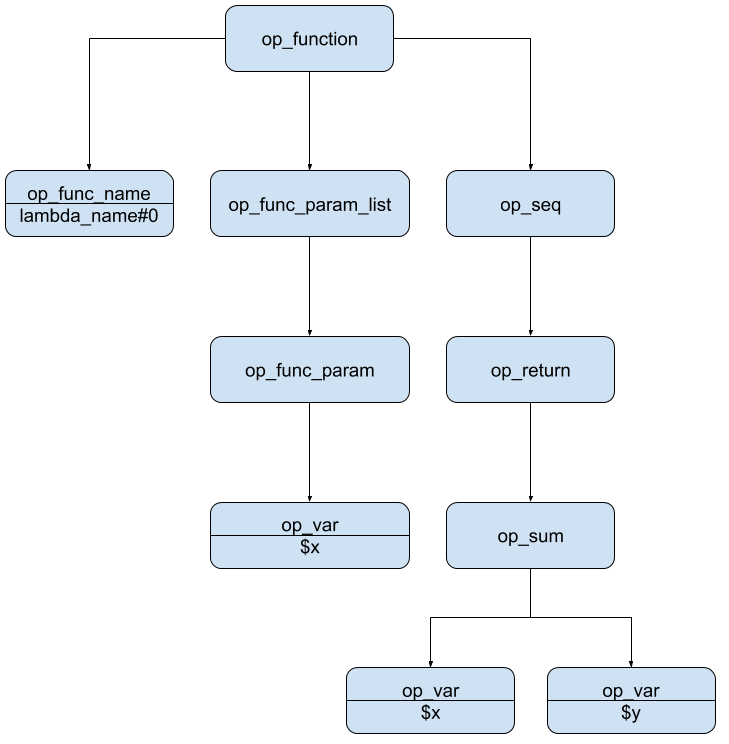
\includegraphics[width=\linewidth]{images/ast_for_id}
\end{figure}

Так как каждая анонимная функция должна иметь уникальное имя, будем его генерировать по следующему алгоритму:
\begin{itemize}
  \item возьмем имя текущей функции, которую обрабатываем;
  \item посчитаем от этого имени хеш-функцию;
  \item заведем для каждой функции индивидуальный счетчик и попросим следующее число;
  \item новое имя будет конкатенацией результата хеш-функции и полученного числа из счетчика.
\end{itemize}

Такой подход позволяет без блокировок в других потоках, создавать уникальные для всей программы имена анонимных функций.
Когда построено \verb|AST| для данной анонимной функции, теперь надо придумать, куда и как его преобразовывать для дальнейшей работы.

\subsection{Шаблонные функции}
\label{sec:template_functions}
Так как программа, написанная на языке KPHP, транслируется в строго типизированный язык, необходимо придумать механизм для реализации функций высших порядков.
В текущий момент, как было показано в \ref{sec2:runtime_principle}, в языке нет возможности сохранять в одну переменную экземпляры разных классов, то нужно придумать механизм, благодаря которому было бы возможным передавать экземпляры разных классов в одну переменную.

Попробуем сделать такую функцию шаблонную в смысле языка C++.
Тогда возникнет необходимость выносить все реализации таких функций в \verb|header| файлы, что увеличит время компиляции.
Более важным фактором в данной ситуации является то, что теперь нельзя будет больше на уровне компилятора понимать какой тип у той или иной переменной.
KPHP буде не в состоянии проводить статический анализ, так как теряется информация о типах.
Из-за перекладывания задачи работы с шаблонными типами на GCC \cite{gcc} теряется огромный спектр работы с кодом, его оптимизации и выводом ошибок во время компиляции KPHP.

Рассмотрим другой подход, в котором будет произведена мономорфизация для всех шаблонных функций.
Но для начала следует понимать, какие функции шаблонные, а какие нет.
Для этого заведем соответствующую аннотацию \verb|@kphp-template|, которой будем помечать функции в коде.
Так как бывает полезно ссылаться на шаблонный тип, то разрешим указывать название, по которому можно было бы обращаться к этому типу.
Покажем пример шаблонной функции в листинге \ref{lst:kphp-template-id-example}.
В данной функции буквой \verb|T| ссылаемся на тип переданной переменной,  а в качестве возвращаемого значения говорим, что будет значение такого же типа.
Компилятор будет обязан проверить все наложенные ограничения на данный шаблонный тип.
\begin{lstlisting}[caption={Пример функции id, с применением шаблонов},label={lst:kphp-template-id-example}]
/**
 * @kphp-template T $x
 * @kphp-return T
 */
function id($x) {
  return $x;
}
\end{lstlisting}

Для того, чтобы ограничить тип так, что принимаемые две переменные строго одного шаблонного типа, то нужно перечислить все эти переменные через запятую, например, \verb|@kphp-template T $x, $y|.
При попытке передать аргументы разных типов, компилятор выдаст сообщение, содержащие ошибку в данном месте.
Рассмотрим пример, в котором мы возвращаем поле шаблонного аргумента:
\begin{lstlisting}[caption={Пример функции id, с применением шаблонов},label={lst:kphp-dependent-template-example}]
/**
 * @kphp-template WithFooT $x, $y
 * @kphp-template WithBarT $z
 * @kphp-return WithBarT::bar
 */
function id($x, $y, $z) {
  $z->bar = $x->foo() + $y->foo();
  return $z->bar;
}
\end{lstlisting}

В листинге \ref{lst:kphp-dependent-template-example} показано как можно обращаться к типам, которые имеют поля класса, переданного в качестве шаблонного типа.
Также показана возможность ограничения переменных одинаковым типом.
Для того, чтобы принимать лямбда-функции данный синтаксис выглядит слишком многословным.
Воспользуемся тем фактором, что в PHP есть подсказки типов для переменных и добавим в наш язык еще одно ключевое слово -- \verb|callable|.
Следующий пример демонстрирует, как следует писать функции высших порядков, в данном случае \verb|callable| -- синоним для \verb|kphp-template|:
\begin{lstlisting}[caption={Пример использования ключевого слова callable},label={lst:callable_support}]
function apply(callable $sum, $x, $y) {
  return $sum($x, $y);
}

apply(function ($x, $y) { return $x + $y; }, 10, 20);
apply(function ($x, $y) { return (string) ($x * $y); }, 10, 20);
\end{lstlisting}

Теперь необходимо придумать, как поддержать данную семантику.
Так для каждого конкретного вызова функции нам нужно понять от какого типа она вызывается.
В KPHP существует такая сущность как \verb|assumptions| -- это предположения о типах переменных до вывода типов, зачастую при разработке необходимо знать, является ли данное выражение примитивным типом или это класс.
Также нужно понимать какой это класс, в конце работы компилятора, после вывода типов, KPHP снова проверяет совпали ли сделанные предположения с конечным выведенным типом.
Воспользуемся этим при реализации шаблонных функций.

К моменту вывода типов необходимо расставить все необходимые ссылки на вызовы функций.
Встроимся в этап \verb|Process Function| (см. рисунок \ref{fig:compiler_arch}).
Для каждой вершины \verb|op_func_call| постараемся привязать соответствующую функцию, если понимаем, что она шаблонная то выводим предположения о типах и генерируем новую функцию.
Так поступаем с каждым вызовом, нам нужно клонировать функцию, подменив ей имя и обновить текущий вызов.
Рассмотрим пример сгенерированного кода на C++ который был получен путем запуска KPHP на коде из листинга \ref{lst:callable_support}:
\begin{lstlisting}
int apply_lambda0(class_instance<lambda0> sum, int x, int y) {
  return lambda0_invoke(sum, x, y);
}

string apply_lambda1(class_instance<lambda1> sum, int x, int y) {
  return lambda1_invoke(sum, x, y);
}

apply_lambda0(lambda0_construct(), 10, 20);
apply_lambda1(lambda1_construct(), 10, 20);
\end{lstlisting}

\subsection{Вывод типов}
Рассмотрим, как должен происходить вывод типов.
Все параметры лямбда-функции будут иметь шаблонный тип такой, что можно принять любую лямбда-функцию, либо класс, у которого есть метод \verb|__invoke|.
На самом деле анонимная функция представляет из себя класс, у которого есть метод \verb|__invoke|.

Рассмотрим, как выводятся типы результата вызова лямбда-функции и типы во встроенных функциях.
Так как все вызовы лямбда функции транслируются просто в вызов соответствующего метода, то тут все будет работать из коробки.
\verb|KPHP| умел до этого выводить типы для вызова методов конкретного класса.
Но нужно добавить поддержку для вывода типов встроенных методов, в которые передают лямбда-функции.

Теперь необходимо разработать аннотацию для встроенных функций.
Рассмотрим, например, функцию \verb|array_reduce($array, $callback, [$initial])|, которая принимает массив, функцию с помощью которой она будет выполнять левоассоциативную свертку \cite{foldl} и начальное значение.
Например \verb|array_reduce([1, 2], sum, 10);| -- возьмет начальное значение 10 и добавит к нему по очереди элементы массива один и два, в результате получим число 13.

Функция \verb|array_reduce| принимает первым аргументов массив каких-либо значений, запишем тип массива, хранящий любые однородные значения в следующем виде: \verb|array<Any>|.
Следующий аргумент -- это другая функция, попробуй подумать какой у нее может быть тип:
\begin{enumerate}
  \item первый аргумент ее может принимать начальное значение, передаваемое третьим аргументом;
  \item первый аргумент может принимать значения, которая вернула сама функция свертки;
  \item вторым аргументом она всегда принимает значения из переданного массива;
  \item возвращает любое значение.
\end{enumerate}

Формализуем описанные выше требования.
Введем по аналогии с \verb|PHP| ключевое слово для типа принимаемой функции -- \verb|callback|.
Функция которую мы принимаем для свертки будет выглядеть следующим образом: \verb|callback($carry, $item) ::: Any|.
Синтаксис \verb|:::| -- ограничивает выражение стоящее слева от него соответствующим типом, то есть наша функция может вернуть все что угодно.
Параметр \verb|$carry| будет иметь тип \verb|lca<^3, ^2()>|.
Слово \verb|lca| в данном контексте означает такой тип, который может содержать любые значения, из типа \verb|^3| и типа \verb|^2()|.
\verb|^3| -- это ссылка на 3 аргумент функции, формально она говорит возьми тот тип, который имеет третий аргумент функции \verb|array_reduce| в данном случае это будет тип переменной \verb|$initial|.
Тип результата вызовы функции обозначим как \verb|^2()| -- это результат вызова функции, передаваемой вторым аргументом, то есть функции для свертки.
Также наша функция принимает аргумент \verb|$item|, который будет иметь тип такой же, как и элемент массива, то есть \verb|^1[]|.

Нам осталось только добавить тип для переменной, задающей начальное значение -- \verb|$initial|, так как она может быть какой угодно то ей зададим тип \verb|Any|,  а возвращаемый тип всей функции будет такой же, какой имеет параметр \verb|$carry| нашей функции, то есть \verb|lca<^3, ^2()>|.
Полный пример для указания типа функции \verb|array_reduce| представлен в листинге \ref{lst:typed_array_reduce}.
\begin{lstlisting}[caption={Пример типизации функции array\_reduce},label={lst:typed_array_reduce}]
function array_reduce(
  $a ::: array,
  callback($carry ::: lca<^3, ^2()>, $item ::: ^1[]) ::: Any,
  $initial ::: Any) ::: lca<^3, ^2()>;
\end{lstlisting}

Далее в качестве примера приведем типизации для нескольких встроенных функций \verb|array_filter| -- листинг \ref{lst:typed_array_filter}, \verb|array_map| -- листинг \ref{lst:typed_array_map} и \verb|usort| представлен в листинге \ref{lst:typed_usort}.
\begin{lstlisting}[caption={Пример типизации функции array\_filter},label={lst:typed_array_filter}]
function array_filter(
  $a ::: array,
  callback ($x ::: ^1[]) ::: bool = DEFAULT) ::: ^1;
\end{lstlisting}
\begin{lstlisting}[caption={Пример типизации функции array\_map},label={lst:typed_array_map}]
function array_map(
  callback ($x ::: ^2[]) ::: Any,
  $a ::: array) ::: array <^1()>;
\end{lstlisting}
\begin{lstlisting}[caption={Пример типизации функции usort},label={lst:typed_usort}]
function usort(
  &$a ::: array,
  callback($x ::: ^1[], $y ::: ^1[]) ::: int) ::: void;
\end{lstlisting}

Для вывода типов сначала нужно разобрать придуманный нами синтаксис и представить его в удобной форме.
Будем использовать \verb|enum-тип|, каждое значение которого обозначает какой-либо примитивный тип:
\begin{lstlisting}
enum PrimitiveType {
  tp_Unknown,
  tp_False,
  tp_bool,
  tp_int,
  tp_float,
  tp_array,
  tp_string,
  tp_void,
  tp_var,
  tp_Class,
  tp_Error,
  tp_Any,
};
\end{lstlisting}

Построим дерево, обозначающее данный тип, например, для функции \verb|array_map|, в которую передают только анонимную функцию:
\begin{lstlisting}[label={lst:array_map_typed_ast}]
function array_map(
  callback($x ::: ^2[]) ::: Any
) ::: array<^1()>;
\end{lstlisting}
Мы получим дерево, изображенное на рисунке \ref{fig:ast_for_callback}.
Строим обычное дерево для функции, оно представлено слева, для упрощения убраны лишние вершины.
В каждой вершине есть поле \verb|type_rule| которое заполняется по мере необходимости.
Так, например, мы видим, что возвращаемое значение функции \verb|array_map|, содержащиеся в поле \verb|type_rule| вершины \verb|op_function|, представляет из себя массив элементов, которые имеют тип такой же, как и результат вызова первого параметра.

\begin{figure}[H]
    \caption{Дерево разбора для типизации функции из листинга \ref{lst:array_map_typed_ast}}
    \label{fig:ast_for_callback}
    \centering
    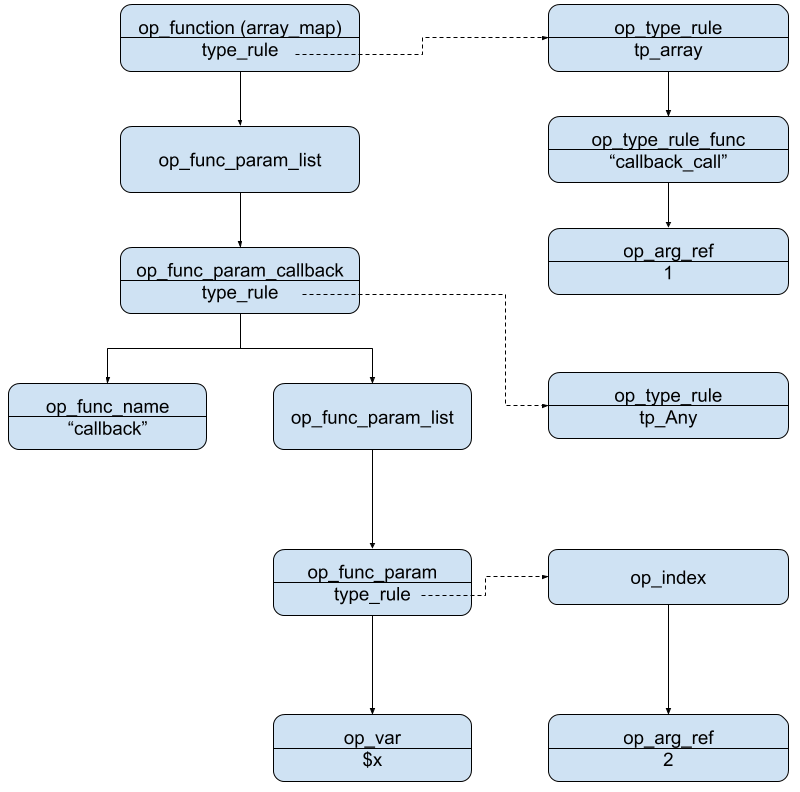
\includegraphics[width=\linewidth]{images/ast_for_callback}
\end{figure}

Осталось лишь встроить нужную логику в \verb|Type Inferencer| (см. рисунок \ref{fig:compiler_arch}).
Во время вывода типов, для каждого выражения устанавливаются ограничения, что тип одного выражения должен иметь как минимум тип другого.
Например в выражении \verb|$x = foo();| ставится ограничение, что переменная должна иметь тип содержащий в себе множество значений не меньшее, чем множество содержащиеся в типе возвращаемого значения функции.
Таким образом, если в поле \verb|type_rule| при нахождении ``callback\_call'', содержащийся в вершине \verb|op_type_rule_func| -- то необходимо достать нужный функциональный тип по порядковому номеру.
На текущее выражение будем накладывать ограничение, что оно должно иметь тип как минимум такой, какой имеет возвращаемое значение данной функции.

Также при задании типов аргументов \verb|callback|, надо наложить соответствующие ограничения.
То есть берется переданная функция, достаем типы, указанные в аннотации к функции, и говорим, что данный параметр, переданной функции имеет как минимум такой тип.
Так же поступаем и с возвращаемым аргументом лямбда-функции.

\subsection{Кодогенерация}
В \verb|PHP| один из магических методов в классе является \verb|__invoke|, если класс имеет этот метод, то \verb|PHP| гарантирует, что при попытке вызвать экземпляр данного класса, передав ему аргументы он вызовет данный метод.
Лямбда-функции преобразовываются в соответствующей класс и глобальный метод \verb|__invoke|, который принимает в качестве первого аргумента экземпляр самой лямбда-функции.
Все захваченные переменные становятся полями данного класса.

Рассмотрим пример генерации функции, которая складывает передаваемое ей число и захваченную глобальную переменную:
\begin{lstlisting}[label={lst:sum_x_captured},caption={Пример функции, добавляющей к аргументу захваченное значение}]
$y = 8;

$add_y = function ($x) use ($y) {
  return $x + $y;
};

$add_y(228);
\end{lstlisting}

Для лямбда-функции, приведенной в листинге \ref{lst:sum_x_captured}, будет сгенерирован следующий класс:
\begin{lstlisting}
struct lambda1 final : refcountable_php_classes<lambda1> {
  int y;
};
\end{lstlisting}

Также будут сгенерированы глобальные методы для конструирования данной лямбда-функции и вызова соответствующего \verb|__invoke| метода:
\begin{lstlisting}
class_instance<lambda1> lambda1_construct(int y) {
  class_instance<lambda1> lambda1_this;
  lambda1_this.alloc();

  lambda1_this->y = y;
  return lambda1_this;
}

int lambda1_invoke_not_instance(class_instance<lambda1> const &lambda1_this, int x) {
  return x + lambda1_this->$y;
}
\end{lstlisting}

Код из листинга \ref{lst:sum_x_captured} будет преобразован, с использованием полученных классов и функций, в следующий:
\begin{lstlisting}
int y = 8;
class_instance<lambda1> id = lambda1_construct(y);
lambda1_invoke_not_instance(id, 228);
\end{lstlisting}

Данный подход генерации лямбда-функций удобен тем, что удачно вписывается в текущую архитектуру кодогенерации \verb|KPHP|.

\section{Поддержка интерфейсов}
Для того чтобы иметь возможность сохранять разные лямбда-функции в одну и туже переменную, но которые имеют схожую сигнатуру, необходимо разработать новую сущность, позволяющую обобщать классы.
Сейчас нет возможности в языке сохранять различные классы в одну и туже переменную, однако интерфейсы смогут разрешить эту проблему.
После чего можно будет придумать специальный синтаксис для аннотации таких переменных, что позволит сохранять в поля класса разные экземпляры лямбда-функций.
Также появится возможность сохранять в одну и туже переменную разные анонимные функции.

\subsection{Разбор синтаксиса}
Рассмотрим, как выглядят интерфейсы в языке PHP.
Они начинаются с ключевого слова \verb|interface|, каждый интерфейс имеет уникальное имя.
Внутри мы можем определять константы, статические функции и методы, которые должны быть обязательно реализованы наследниками.
Рассмотрим пример интерфейса \verb|CallableInterface|:
\begin{lstlisting}[caption={Пример интерфейса Callable},label={lst:callable-interface-example}]
interface CallableInterface {
  public function invoke($x);
}
\end{lstlisting}

Чтобы реализовать интерфейс, необходимо создать класс, указать, что он \verb|implements CallableInterface| и реализовать необходимые функции.
Рассмотрим пример для интерфейса, приведенного в листинге \ref{lst:callable-interface-example}:
\begin{lstlisting}
class PlusFive implements CallableInterface {
  public function invoke($x) {
    return $x + 5;
  } 
}
\end{lstlisting}

Для того, чтобы указать, что переменная реализует данный интерфейс -- нужно написать \verb|PHPDoc| \cite{phpdoc} над переменной \verb|@var CallableInterface|.
Для принимаемых параметров функции по-прежнему работает подсказка типа в параметрах функции.
Также необходимо добавить возможно наследования интерфейсов.
наследование реализуется путем копирования всех методов из родительского интерфейса в дочерней синтаксис для наследования интерфейсов:
\begin{lstlisting}
interface FooInterface {
  public function foo($x);
}

interface BarInterface extends FooInterface {
  public function bar($x, $y);
}

class FooBarClass implements BarInterface {
  public function foo($x) { return $x; }
  public function bar($x, $y) { return $x + $y; }
}
\end{lstlisting}

Также при объявлении интерфейсов у нас бывают аргументы по умолчанию, это нужно учесть.
Причем у наследника у нас может быть больше аргументов, чем у родителя, если они имеют значения по умолчанию.
Также все аргументы, которые у интерфейса имеют значения по умолчанию должны иметь одинаковые значения в наследниках.

Далее нам понадобится механизм для проверки, является ли данное выражение, представляющее базовый класс, классом-наследником.
Это будет осуществляться с помощью оператора \verb|instanceof|.
Введем также дополнительную функцию \verb|instance_cast|, для понижающего приведения.
Однако так как в \verb|PHP| используется динамическая типизация, становится неудобным сначала проверять на \verb|instanceof|, а после производить \verb|instance_cast|.
Давайте для этого заведем состояние для каждой переменной, участвовавшей в условии на \verb|instanceof| и в зависимости от состояния, будем производить нужное приведение типов.
В листинге \ref{lst:smart_instanceof} показано как должно происходить автоматическое понимание какого типа на самом деле является переменная.
\begin{lstlisting}[caption={Пример использования умного оператора instanceof},label={lst:smart_instanceof}]
interface I { public function print_i(); }

interface IA extends I { public function print_ia(); }
interface IB extends I { public function print_ib(); }

class A implements IA {
    public function print_i() { var_dump("print_i::A"); }
    public function print_ia() { var_dump("print_ia::A"); }

    public function _a() { var_dump("_a"); }
}

class B implements IA {
    public function print_i() { var_dump("print_i::B"); }
    public function print_ia() { var_dump("print_ia::B"); }

    public function _b() { var_dump("_b"); }
}

class C implements IB {
    public function print_i() { var_dump("print_i::C"); }
    public function print_ib() { var_dump("print_ib::C"); }

    public function _c() {
        var_dump("_c");
    }
}

function call_method(I $x) {
  $x->print_i();
  if ($x instanceof IA) {
      $x->print_ia();
      if ($x instanceof A) {
          $x->_a();
          $x->_a();
      } else {                # $x is B
          $x->_b();
      }
  } else {                    # $x is IB
      $x->print_ib();
      if ($x instanceof C) {
          $x->_c();
      }
  }
}
\end{lstlisting}

В листинге \ref{lst:smart_instanceof} отображена работа с интерфейсами, которые были реализованы в рамках написания данной работы.
Данный код корректный и KPHP понимает в какой из областей видимости возможны варианты для типа переменной.
Это было реализовано при помощи поддержки состояний для каждой переменной и анализа CFG.

\subsection{Генерация методов}
Рассмотрим, как происходит преобразование интерфейсных методов.
Для каждого класса заведем новое поле, содержащее множество интерфейсов, которые он реализует.
Собственно, для каждого интерфейса будем хранить множество классов, которые его реализует.
В отдельной стадии компиляции пробежимся по всем интерфейсным функциям и сгенерируем код, который будет проверять на принадлежность одному из подклассов и вызывать нужный метод.
Приведем пример в листинге \ref{lst:interface-method-example} для генерации метода \verb|print_ia| для интерфейса \verb|IA| из листинга \ref{lst:smart_instanceof}.
\begin{lstlisting}[caption={Пример генерации интерфейсного метода},label={lst:interface-method-example}]
function print_ia($vthis) {
  if ($vthis instanceof A) {
    return $vthis->print_ia();
  } else {
    return $vthis->print_ia();
  }
}
\end{lstlisting}

При реализации методов интерфейсов было рассмотрено несколько вариантов.
Один из них, это генерировать код как настоящие методы в C++ классы и соответственно реализовывать интерфейсы через обычное наследование средствами языка C++.
Появилась гарантия правильности аргументов и возвращаемых значений.
Также то что должно было быть переопределено будет чисто-виртуальным методом.
Однако такой подход имеет свои недостатки, так как в C++ разрешается иметь только ковариантные возвращаемые значения.
Однако мы не можем иметь контравариантные принимаемые значение, что вполне логично для языка PHP.

Было принято решение, генерировать такие методы как обычные глобальные функции, принимающие первым аргументом указатель на интерфейс.
Вывод типов автоматически справится либо обобщить возвращаемый тип интерфейсного метода, либо наоборот сузить его в методах наследников.
Но для совершения понижающего приведения все еще необходима иерархия наследования, поэтому логично совместить два подхода.
Будем наследовать классы от интерфейсов, но методы будем создавать отдельно.

Так как интерфейсы, как и другие классы должны реализовывать ссылочную семантику, то нужно выделить только один счетчик ссылок на всю иерархию наследования, чтобы не происходило двойного удаления или же утечек памяти.
При генерации кода будем проверять, реализует ли наш класс какой-либо интерфейс и в зависимости от этого будем его наследовать либо от класса с простым подсчетом ссылок, либо от класса, который переопределит родительские функции для подсчета.
Так как счетчик должен будет реализовывать нужные функции, которые находятся в интерфейсе, то передаем его через CRTP \cite{crtp}, тем самым он сможет продлить иерархию унаследовав себя от нужного интерфейса.
Рассмотрим, что получится при генерации интерфейсных классов, для примера, приведенного в листинге \ref{lst:smart_instanceof}:
\begin{lstlisting}
class abstract_refcountable_php_interface {
public:
  virtual ~abstract_refcountable_php_interface() = default;
  virtual void add_ref() = 0;
  virtual void release() = 0;
  virtual uint32_t get_refcnt() = 0;
  virtual void set_refcnt(uint32_t new_refcnt) = 0;
};

template<class Derived, class Base = void>
class refcountable_php_classes : public Base {
public:
  void add_ref() final {...}
  uint32_t get_refcnt() final {...}
  void release() final {...}
  void set_refcnt(uint32_t new_refcnt) final {...}

private:
  uint32_t refcnt{0};
};


struct I : public abstract_refcountable_php_interface {};
struct IA : public I {};
struct A final : public refcountable_php_classes<A, IA> {};
struct B final : public refcountable_php_classes<B, IA> {};
\end{lstlisting}

Для создания понижающего приведения надо будет воспользоваться \verb|dynamic_cast| и созданием нужного класса из этого указателя.
При выводе типов переменных необходимо отслеживать какие классы присваиваются и находить их наименьшего общего предка \cite{lca}, что позволит указать данному выражению найденный тип.

\subsection{Лямбда-функции как члены классов}
В текущий момент имеем реализацию интерфейсов и необходимо на ее основе построить возможность сохранения несколько лямбда-функций в одну переменную.
Приведем пример того, как это можно было бы сделать, не используя лямбда-функции в листинге \ref{lst:lambda-as-field-example}.
\begin{lstlisting}[caption={Пример замены сохранения лямбда-функции в поле класса},label={lst:lambda-as-field-example}]
interface ApplyInterface {
    public function invoke($x, $y);
}

class Sum implements ApplyInterface {
    public function invoke($x, $y) {
        return $x + $y;
    }
}

class Mul implements ApplyInterface {
    public function invoke($x, $y) {
        return $x * $y;
    }
}

class LambdaHolder {
    /** @var ApplyInterface */
    public $lambda = false;

    public function use_lambda($x, $y) {
        var_dump($this->lambda->invoke($x, $y));
    }
}

$lambda_holder = new LambdaHolder();
$lambda_holder->lambda = new Sum();
$lambda_holder->use_lambda(10, 20);

$lambda_holder->lambda = new Mul();
$lambda_holder->use_lambda(10, 20);
\end{lstlisting}

Данный синтаксис многословен, но он не уступает по функциональным возможностям лямбда-функциям, сохраненных в поля класса.
Осталось только разработать синтаксис для аннотации полей классов, что они будут содержать анонимные функции с определенным количеством аргументов.
Тогда можно будет все передаваемый лямбда-функции автоматически наследовать от сгенерированного интерфейса и сохранять в поля класса и переменные, но это еще не было реализовано.
Поэтому в данном случае нам придется пожертвовать красотой и быть многословными, однако данная работа уже запланирована.

\chapterconclusion
В данной главе познакомились с языком KPHP и разобрались, как работают его основные составляющие: компилятор и рантайм.
Разобрались с архитектурой, что помогло дополнить нужные части языка необходимым функционалом.
Посмотрели на пример анонимных функции и с какими сложностями нам пришлось столкнуться.
Была представлена техническая сложность реализации, поставленной перед нами задачи.
Добавили новую сущность в KPHP -- шаблонных функции, благодаря которым нам удалось реализовать функции высших порядков.
Разработан синтаксис для типизации встроенных функций, принимающих лямбда-функции.
Были рассмотрены аспекты и необходимые технические детали для того, чтобы сохранять разные анонимные функции в члены классов и переменные.
Для этого необходимо было реализовать интерфейсы в языке и необходимую инфраструктуру.

В следующей главе будет приведен анализ и сравнение получившегося решения с аналогичными в языках Hack и PHP.
Также увидим, что спроектированное и реализованное решение не накладывает дополнительных расходов.
